%

\documentclass[mathserif]{beamer}


% This file is a solution template for:

% - Giving a talk on some subject.
% - The talk is between 15min and 45min long.
% - Style is ornate.

% Copyright 2004 by Till Tantau <tantau@users.sourceforge.net>.
%
% In principle, this file can be redistributed and/or modified under
% the terms of the GNU Public License, version 2.
%
% However, this file is supposed to be a template to be modified
% for your own needs. For this reason, if you use this file as a
% template and not specifically distribute it as part of a another
% package/program, I grant the extra permission to freely copy and
% modify this file as you see fit and even to delete this copyright
% notice.
\usepackage{graphicx, graphics}
\usepackage[english]{babel}
%

%%%%%%%%%%%%%%%%%%%%%%%%%%%%%%%%%%%%%%%%%%%%%%%%%%%%%%%%%%%%%%%%%%
% General
%%%%%%%%%%%%%%%%%%%%%%%%%%%%%%%%%%%%%%%%%%%%%%%%%%%%%%%%%%%%%%%%%%
\newfont{\msym}{msbm10}
\newcommand{\reals}{\mathbb{R}}%Re}%{mbox{\msym R}}
\newcommand{\half}{\frac{1}{2}}       
\newcommand{\sign}{{\rm sign}}
\newcommand{\paren}[1]{\left({#1}\right)}
\newcommand{\brackets}[1]{\left[{#1}\right]}
\newcommand{\braces}[1]{\left\{{#1}\right\}}
\newcommand{\ceiling}[1]{\left\lceil{#1}\right\rceil}
\newcommand{\abs}[1]{\left\vert{#1}\right\vert}
\newcommand{\tr}{{\rm Tr}}
\newcommand{\pr}[1]{{\rm Pr}\left[{#1}\right]}
\newcommand{\prp}[2]{{\rm Pr}_{#1}\left[{#2}\right]}
\newcommand{\Exp}[1]{{\rm E}\left[{#1}\right]}
\newcommand{\Expp}[2]{{\rm E}_{#1}\left[{#2}\right]}
\newcommand{\eqdef}{\stackrel{\rm def}{=}}
\newcommand{\comdots}{, \ldots ,}
\newcommand{\true}{\texttt{True}}
\newcommand{\false}{\texttt{False}}
\newcommand{\mcal}[1]{{\mathcal{#1}}}
\newcommand{\argmin}[1]{\underset{#1}{\mathrm{argmin}} \:}
\newcommand{\normt}[1]{\left\Vert {#1} \right\Vert^2}
\newcommand{\step}[1]{\left[#1\right]_+}
\newcommand{\1}[1]{[\![{#1}]\!]}
\newcommand{\diag}{{\textrm{diag}}}
%\newcommand{\det}{{\textrm{det}}}
\newcommand{\KL}{{\textrm{D}_{\textrm{KL}}}}
\newcommand{\IS}{{\textrm{D}_{\textrm{IS}}}}
\newcommand{\EU}{{\textrm{D}_{\textrm{EU}}}}
\newcommand{\lloss}{\ell} % label loss
\newcommand{\closs}{\hat\ell} % classifier loss
\newcommand{\st}{\textrm{s.t.}} % such that / subject to

%%%%%%%%%%%%%%%%%%%%%%%%%%%%%%%%%%%%%%%%%%%%%%%%%%%%%%%%%%
% Control symbols
%%%%%%%%%%%%%%%%%%%%%%%%%%%%%%%%%%%%%%%%%%%%%%%%%%%%%%%%%%
\newcommand{\leftmarginpar}[1]{\marginpar[#1]{}}
\newcommand{\figline}{\rule{0.50\textwidth}{0.5pt}}
\newcommand{\pseudocodefont}{\normalsize}
\newcommand{\nolineskips}{
\setlength{\parskip}{0pt}
\setlength{\parsep}{0pt}
\setlength{\topsep}{0pt}
\setlength{\partopsep}{0pt}
\setlength{\itemsep}{0pt}}

%%%%%%%%%%%%%%%%%%%%%%%%%%%%%%%%%%%%%%%%%%%%%%%%%%%%%%%%%%%
% Equations and references
%%%%%%%%%%%%%%%%%%%%%%%%%%%%%%%%%%%%%%%%%%%%%%%%%%%%%%%%%%%
\newcommand{\beq}[1]{\begin{equation}\label{#1}}
\newcommand{\eeq}{\end{equation}}
\newcommand{\beqa}{\begin{eqnarray}}
\newcommand{\eeqa}{\end{eqnarray}}
%\renewcommand{\eqref}[1]{Eq.~(\ref{#1})}
\newcommand{\exmref}[1]{Example~\ref{#1}} 
\newcommand{\sthmref}[1]{Thm.~\ref{#1}}  
\newcommand{\remref}[1]{Remark~\ref{#1}} 
\newcommand{\claimref}[1]{Claim~\ref{#1}} 
\newcommand{\corref}[1]{Corollary~\ref{#1}} 
\newcommand{\scorref}[1]{Cor.~\ref{#1}} 
\newcommand{\tran}[1]{{#1}^{\top}}
\newcommand{\norm}{\mcal{N}}
\newcommand{\eqsref}[1]{Eqns.~(\ref{#1})}

% Alex's macros

\newcommand{\chaplabel}[1]{\label{chap:#1}}
\newcommand{\chapref}[1]{Chapter~\ref{chap:#1}}

\newcommand{\seclabel}[1]{\label{sec:#1}}
\newcommand{\secref}[1]{Section~\ref{sec:#1}}

\newcommand{\applabel}[1]{\label{app:#1}}
\newcommand{\appref}[1]{Appendix~\ref{app:#1}} 

\newcommand{\figlabel}[1]{\label{fig:#1}}
\newcommand{\figref}[1]{Figure~\ref{fig:#1}}

\newcommand{\tablabel}[1]{\label{tab:#1}}
\newcommand{\tabref}[1]{Table~\ref{tab:#1}}

\newcommand{\eqlabel}[1]{\label{eq:#1}}
\renewcommand{\eqref}[1]{Equation~(\ref{eq:#1})}

\newcommand{\proplabel}[1]{\label{prop:#1}}
\newcommand{\propref}[1]{Proposition~\ref{prop:#1}}

\newcommand{\deflabel}[1]{\label{def:#1}}
\newcommand{\defref}[1]{Definition~\ref{def:#1}}

\newcommand{\lemlabel}[1]{\label{lem:#1}}
\newcommand{\lemref}[1]{Lemma~\ref{lem:#1}}

\newcommand{\thmlabel}[1]{\label{thm:#1}}
\newcommand{\thmref}[1]{Theorem~\ref{thm:#1}}

\newcommand{\alglabel}[1]{\label{alg:#1}}
\newcommand{\algref}[1]{Algorithm~\ref{alg:#1}}


%%%%%%%%%%%%%%%%%%%%%%%%%%%%%%%%%%%%%%%%%%%%%%%%%%%%%%%%%%%
% bold, up, down
%%%%%%%%%%%%%%%%%%%%%%%%%%%%%%%%%%%%%%%%%%%%%%%%%%%%%%%%%%%
\newcommand{\mb}[1]{{\boldsymbol{#1}}}
\newcommand{\up}[2]{{#1}^{#2}}
\newcommand{\dn}[2]{{#1}_{#2}}
\newcommand{\du}[3]{{#1}_{#2}^{#3}}
\renewcommand{\star}[1]{\up{#1}{*}}
\newcommand{\textl}[2]{{$\textrm{#1}_{\textrm{#2}}$}}


%%%%%%%%%%%%%%%%%%%%%%%%%%%%%%%%%%%%%%%%%%%%%%%%%%%%%%%%%%%
% vectors \va
%%%%%%%%%%%%%%%%%%%%%%%%%%%%%%%%%%%%%%%%%%%%%%%%%%%%%%%%%%%
\newcommand{\vx}{\mb{x}} 
\newcommand{\vxi}[1]{\vx_{#1}}
\newcommand{\vxii}{\vxi{i}}

\newcommand{\yi}[1]{y_{#1}}
\newcommand{\yii}{\yi{i}}
\newcommand{\hy}{\hat{y}}
\newcommand{\hyi}[1]{\hat{y}_{#1}}
\newcommand{\hyii}{\hyi{i}}

\newcommand{\vy}{\mb{y}} 
\newcommand{\vyi}[1]{\vy_{#1}}
\newcommand{\vyii}{\vyi{i}}

\newcommand{\vn}{\mb{\nu}} 
\newcommand{\vni}[1]{\vn_{#1}}
\newcommand{\vnii}{\vni{i}}

\newcommand{\vmu}{\mb{\mu}}
\newcommand{\vmus}{{\vmu^*}}
\newcommand{\vmuts}{{\vmus}^{\top}}
\newcommand{\vmui}[1]{\vmu_{#1}}
\newcommand{\vmuii}{\vmui{i}}

\newcommand{\vmut}{\vmu^{\top}}
\newcommand{\vmuti}[1]{\vmut_{#1}}
\newcommand{\vmutii}{\vmuti{i}}

\newcommand{\vsigma}{\mb \sigma}
\newcommand{\msigma}{\Sigma}
\newcommand{\msigmas}{{\msigma^*}}
\newcommand{\msigmai}[1]{\msigma_{#1}}
\newcommand{\msigmaii}{\msigmai{i}}

\newcommand{\mups}{\Upsilon}
\newcommand{\mupss}{{\mups^*}}
\newcommand{\mupsi}[1]{\mups_{#1}}
\newcommand{\mupsii}{\mupsi{i}}
\newcommand{\upssl}{\upsilon^*_l}


\newcommand{\vu}{\mb{u}} 
\newcommand{\vut}{\tran{\vu}}
\newcommand{\vui}[1]{\vu_{#1}}
\newcommand{\vuti}[1]{\vut_{#1}}
\newcommand{\hvu}{\hat{\vu}}
\newcommand{\hvut}{\tran{\hvu}}
\newcommand{\hvur}[1]{\hvu_{#1}}
\newcommand{\hvutr}[1]{\hvut_{#1}}
\newcommand{\vw}{\mb{w}} 
\newcommand{\vwi}[1]{\vw_{#1}}
\newcommand{\vwii}{\vwi{i}}

\newcommand{\vwt}{\tran{\vw}}
\newcommand{\vwti}[1]{\vwt_{#1}}
\newcommand{\vwtii}{\vwti{i}}

\newcommand{\vv}{\mb{v}} 
\newcommand{\vvt}{\tran{\vv}}

\newcommand{\vvi}[1]{\vv_{#1}}
\newcommand{\vvti}[1]{\vvt_{#1}}
\newcommand{\lambdai}[1]{\lambda_{#1}}
\newcommand{\Lambdai}[1]{\Lambda_{#1}}

\newcommand{\vxt}{\tran{\vx}}
\newcommand{\hvx}{\hat{\vx}}
\newcommand{\hvxi}[1]{\hvx_{#1}}
\newcommand{\hvxii}{\hvxi{i}}
\newcommand{\hvxt}{\tran{\hvx}}
\newcommand{\hvxti}[1]{\hvxt_{#1}}
\newcommand{\hvxtii}{\hvxti{i}}
\newcommand{\vxti}[1]{\vxt_{#1}}
\newcommand{\vxtii}{\vxti{i}}

%%%%%%%%%%%%%%%%%%%%%%%%%%%%%%%%%%%%%%%%%%%%%%%%%%%%%%%%%%%%%%%%%
% Matrices (\mA)
%%%%%%%%%%%%%%%%%%%%%%%%%%%%%%%%%%%%%%%%%%%%%%%%%%%%%%%%%%%%%%%%%


\renewcommand{\mp}{P}
\newcommand{\mpd}{\mp^{(d)}}
\newcommand{\mpt}{\mp^T}
\newcommand{\tmp}{\tilde{\mp}}
\newcommand{\mpi}[1]{\mp_{#1}}
\newcommand{\mpti}[1]{\mpt_{#1}}
\newcommand{\mptii}{\mpti{i}}
\newcommand{\mpii}{\mpi{i}}
\newcommand{\mps}{Q}
\newcommand{\mpsi}[1]{\mps_{#1}}
\newcommand{\mpsii}{\mpsi{i}}
\newcommand{\tmpt}{\tmp^T}
\newcommand{\mz}{Z}
\newcommand{\mv}{V}
\newcommand{\mvi}[1]{\mv_{#1}}
\newcommand{\mvt}{V^T}
\newcommand{\mvti}[1]{\mvt_{#1}}
\newcommand{\mzt}{\mz^T}
\newcommand{\tmz}{\tilde{\mz}}
\newcommand{\tmzt}{\tmz^T}
\newcommand{\mx}{\mathbf{X}}
\newcommand{\ma}{\mathbf{A}}
\newcommand{\mxs}[1]{\mx_{#1}}


\newcommand{\mxi}[1]{\textrm{diag}^2\paren{\vxi{#1}}}
\newcommand{\mxii}{\mxi{i}}

%\newcommand{\mxi}[1]{\mx_{#1}}
%\newcommand{\mxii}{\mxi{i}}
\newcommand{\hmx}{\hat{\mx}}
\newcommand{\hmxi}[1]{\hmx_{#1}}
\newcommand{\hmxii}{\hmxi{i}}
\newcommand{\hmxt}{\hmx^T}
\newcommand{\mxt}{\mx^\top}
\newcommand{\mi}{I}
\newcommand{\mq}{Q}
\newcommand{\mqt}{\mq^T}
\newcommand{\mlam}{\Lambda}
%\newcommand{\ma}{A}
%\newcommand{\ms}{S}
%\newcommand{\mt}{T}

%%%%%%%%%%%%%%%%%%%%%%%%%%%%%%%%%%%%%%%%%%%%%%%%%%%%%%%%%%%
% mathcal 
%%%%%%%%%%%%%%%%%%%%%%%%%%%%%%%%%%%%%%%%%%%%%%%%%%%%%%%%%%%
\renewcommand{\L}{\mcal{L}}
\newcommand{\R}{\mcal{R}}
\newcommand{\X}{\mcal{X}}
\newcommand{\Y}{\mcal{Y}}
\newcommand{\F}{\mcal{F}}
\newcommand{\nur}[1]{\nu_{#1}}
\newcommand{\lambdar}[1]{\lambda_{#1}}
\newcommand{\gammai}[1]{\gamma_{#1}}
\newcommand{\gammaii}{\gammai{i}}
\newcommand{\alphai}[1]{\alpha_{#1}}
\newcommand{\alphaii}{\alphai{i}}
\newcommand{\lossp}[1]{\ell_{#1}}
\newcommand{\eps}{\epsilon}
\newcommand{\epss}{\eps^*}
\newcommand{\lsep}{\lossp{\eps}}
\newcommand{\lseps}{\lossp{\epss}}
\newcommand{\T}{\mcal{T}}

%%%%%%%%%%%%%%%%%%%%%%%%%%%%%%%%%%%%%%%%%%%%%%%%%%%%%%%%%%%
% Notes
%%%%%%%%%%%%%%%%%%%%%%%%%%%%%%%%%%%%%%%%%%%%%%%%%%%%%%%%%%%
\newcommand{\kc}[1]{\begin{center}\fbox{\parbox{3in}{{\textcolor{green}{KC: #1}}}}\end{center}}
\newcommand{\fp}[1]{\begin{center}\fbox{\parbox{3in}{{\textcolor{red}{FP: #1}}}}\end{center}}
\newcommand{\md}[1]{\begin{center}\fbox{\parbox{3in}{{\textcolor{blue}{MD: #1}}}}\end{center}}
\newcommand{\ak}[1]{\begin{center}\fbox{\parbox{3in}{{\textcolor{yellow}{AK: #1}}}}\end{center}}




\newcommand{\newstuffa}[2]{#2}
\newcommand{\newstufffroma}[1]{}
\newcommand{\newstufftoa}{}
%\newcommand{\newstuffa}[2]{~\\{\color{MyRed} #1:\\ }{\textcolor{MyGray}{#2}~\\}}
%\newcommand{\newstufffroma}[1]{~\\{\color{MyRed} #1:\\ }\color{MyGray}}
%\newcommand{\newstufftoa}{\color{black}}

\newcommand{\newstuff}[2]{#2}
\newcommand{\newstufffrom}[1]{}
\newcommand{\newstuffto}{}
\newcommand{\oldnote}[2]{}

%%%%\newcommand{\comment}[1]{}
\newcommand{\commentout}[1]{}
\newcommand{\mypar}[1]{\medskip\noindent{\bf #1}}


%%%%%%%%%%%%%%%%%%%%%%%%%%%%%%%%%%%%%%%%%%%%%%%%%%%%%%%%%%%
% other
%%%%%%%%%%%%%%%%%%%%%%%%%%%%%%%%%%%%%%%%%%%%%%%%%%%%%%%%%%%
% inner products
\newcommand{\inner}[2]{\left< {#1} , {#2} \right>}
\newcommand{\kernel}[2]{K\left({#1},{#2} \right)}
\newcommand{\tprr}{\tilde{p}_{rr}}
\newcommand{\hxr}{\hat{x}_{r}}
\newcommand{\projalg}{{PST }}%{\tt Projection }}
\newcommand{\projealg}[1]{$\textrm{PST}_{#1}~$}%{\tt Projection }}
\newcommand{\gradalg}{{GST }}%\tt Gradient }}



\newcounter {mySubCounter}
\newcommand {\twocoleqn}[4]{
  \setcounter {mySubCounter}{0} %
  \let\OldTheEquation \theequation %
  \renewcommand {\theequation }{\OldTheEquation \alph {mySubCounter}}%
  \noindent \hfill%
  \begin{minipage}{.40\textwidth}
\vspace{-0.6cm}
    \begin{equation}\refstepcounter{mySubCounter}
      #1 
    \end {equation}
  \end {minipage}
~~~~~~
%\hfill %
  \addtocounter {equation}{ -1}%
  \begin{minipage}{.40\textwidth}
\vspace{-0.6cm}
    \begin{equation}\refstepcounter{mySubCounter}
      #3 
    \end{equation}
  \end{minipage}%
  \let\theequation\OldTheEquation
}


\newcommand{\vzero}{\mb{0}} 

\newcommand{\smargin}{\mcal{M}}

\newcommand{\ai}[1]{A_{#1}}
\newcommand{\bi}[1]{B_{#1}}
\newcommand{\aii}{\ai{i}}
\newcommand{\bii}{\bi{i}}
\newcommand{\betai}[1]{\beta_{#1}}
\newcommand{\betaii}{\betai{i}}
\newcommand{\mar}{M}
\newcommand{\mari}[1]{\mar_{#1}}
\newcommand{\marii}{\mari{i}}
\newcommand{\nmari}[1]{m_{#1}}
\newcommand{\nmarii}{\nmari{i}}


%\newcommand{\erf}{\mathrm{erf}}
\newcommand{\erf}{\Phi}


\newcommand{\var}{V}
\newcommand{\vari}[1]{\var_{#1}}
\newcommand{\varii}{\vari{i}}

\newcommand{\varb}{v}
\newcommand{\varbi}[1]{\varb_{#1}}
\newcommand{\varbii}{\varbi{i}}

%\newcommand{\vara}{v^+}
\newcommand{\vara}{u}
\newcommand{\varai}[1]{\vara_{#1}}
\newcommand{\varaii}{\varai{i}}

\newcommand{\marb}{m}
\newcommand{\marbi}[1]{\marb_{#1}}
\newcommand{\marbii}{\marbi{i}}

\newcommand{\algname}{{AROW}}
\newcommand{\rlsname}{{RLS}}
\newcommand{\mrlsname}{{MRLS}}


%\newcommand{phi1}{{1+\frac{\phi}{2}}}
\newcommand{\phia}{\psi}
\newcommand{\phib}{\xi}


\newcommand{\amsigmaii}{\tilde{\msigma}_i}
\newcommand{\amsigmai}[1]{\tilde{\msigma}_{#1}}
\newcommand{\avmuii}{\tilde{\vmu}_i}
\newcommand{\avmui}[1]{\tilde{\vmu}_{#1}}
\newcommand{\amarbii}{\tilde{\marb}_i}
\newcommand{\avarbii}{\tilde{\varb}_i}
\newcommand{\avaraii}{\tilde{\vara}_i} 
\newcommand{\aalphaii}{\tilde{\alpha}_i}

\newcommand{\svar}{v}
\newcommand{\smar}{m}
\newcommand{\nsmar}{\bar{m}}

\newcommand{\vnu}{\mb{\nu}}
\newcommand{\vnut}{\vnu^\top}
\newcommand{\vz}{\mb{z}} 
\newcommand{\vZ}{\mb{Z}}
\newcommand{\fphi}{f_{\phi}}
\newcommand{\gphi}{g_{\phi}}

%%% Local Variables: 
%%% mode: latex
%%% TeX-master: "nips2007"
%%% End: 


\newcommand{\vtmui}[1]{\tilde{\vmu}_{#1}}
\newcommand{\vtmuii}{\vtmui{i}}


\newcommand{\zetai}[1]{\zeta_{#1}}
\newcommand{\zetaii}{\zetai{i}}



%%%%%%

\newcommand{\vstate}{\bf{s}}
\newcommand{\vstatet}[1]{\vstate_{#1}}
\newcommand{\vstatett}{\vstatet{t}}

\newcommand{\mtran}{\bf{\Phi}}
\newcommand{\mtrant}[1]{\mtran_{#1}}
\newcommand{\mtrantt}{\mtrant{t}}

\newcommand{\vstatenoise}{\bf{\eta}}
\newcommand{\vstatenoiset}[1]{\vstatenoise_{#1}}
\newcommand{\vstatenoisett}{\vstatenoiset{t}}


\newcommand{\vobser}{\bf{o}}
\newcommand{\vobsert}[1]{\vobser_{#1}}
\newcommand{\vobsertt}{\vobsert{t}}

\newcommand{\mobser}{\bf{H}}
\newcommand{\mobsert}[1]{\mobser_{#1}}
\newcommand{\mobsertt}{\mobsert{t}}

\newcommand{\vobsernoise}{\bf{\nu}}
\newcommand{\vobsernoiset}[1]{\vobsernoise_{#1}}
\newcommand{\vobsernoisett}{\vobsernoiset{t}}

\newcommand{\mstatenoisecov}{\bf{Q}}
\newcommand{\mstatenoisecovt}[1]{\mstatenoisecov_{#1}}
\newcommand{\mstatenoisecovtt}{\mstatenoisecovt{t}}

\newcommand{\mobsernoisecov}{\bf{R}}
\newcommand{\mobsernoisecovt}[1]{\mobsernoisecov_{#1}}
\newcommand{\mobsernoisecovtt}{\mobsernoisecovt{t}}



\newcommand{\vestate}{\bf{\hat{s}}}
\newcommand{\vestatet}[1]{\vestate_{#1}}
\newcommand{\vestatett}{\vestatet{t}}
\newcommand{\vestatept}[1]{\vestatet{#1}^+}
\newcommand{\vestatent}[1]{\vestatet{#1}^-}


\newcommand{\mcovar}{\bf{P}}
\newcommand{\mcovart}[1]{\mcovar_{#1}}
\newcommand{\mcovarpt}[1]{\mcovart{#1}^+}
\newcommand{\mcovarnt}[1]{\mcovart{#1}^-}

\newcommand{\mkalmangain}{\bf{K}}
\newcommand{\mkalmangaint}[1]{\mkalmangain_{#1}}


\newcommand{\vkalmangain}{\bf{\kappa}}
\newcommand{\vkalmangaint}[1]{\vkalmangain_{#1}}



\newcommand{\obsernoise}{{\nu}}
\newcommand{\obsernoiset}[1]{\obsernoise_{#1}}
\newcommand{\obsernoisett}{\obsernoiset{t}}

\newcommand{\obsernoisecov}{r}
\newcommand{\obsernoisecovt}[1]{\obsernoisecov_{#1}}
\newcommand{\obsernoisecovtt}{\obsernoisecov}%t{t}}


\newcommand{\obsnscv}{s}
\newcommand{\obsnscvt}[1]{\obsnscv_{#1}}
\newcommand{\obsnscvtt}{\obsnscvt{t}}


\newcommand{\Psit}[1]{\Psi_{#1}}
\newcommand{\Psitt}{\Psit{t}}

\newcommand{\Omegat}[1]{\Omega_{#1}}
\newcommand{\Omegatt}{\Omegat{t}}


\newcommand{\ellt}[1]{\ell_{#1}}
\newcommand{\gllt}[1]{g_{#1}}

\newcommand{\chit}[1]{\chi_{#1}}

\newcommand{\ms}{\mathcal{M}}
\newcommand{\us}{\mathcal{U}}
\newcommand{\as}{\mathcal{A}}

\newcommand{\mn}{M}
\newcommand{\un}{U}

\newcommand{\set}{S}
\newcommand{\seti}[1]{S_{#1}}

\newcommand{\obj}{\mcal{C}}

%%------------------------------------------------------------------------
%\newcommand {\ebd} {\stackrel{\Delta} {=}}
%\newcommand {\exe} {\stackrel{\cdot} {=}}
%\newcommand{\eqa}{\stackrel{\mbox{(a)}}{=}}
%\newcommand{\eqb}{\stackrel{\mbox{(b)}}{=}}
%\newcommand{\eqc}{\stackrel{\mbox{(c)}}{=}}
%\newcommand{\eqd}{\stackrel{\triangle}{=}}
%\newcommand{\eqe}{\stackrel{\mbox{(e)}}{=}}
%\newcommand{\eqf}{\stackrel{\mbox{(f)}}{=}}
%\newcommand{\lea}{\stackrel{\mbox{(a)}}{\le}}
%\newcommand{\leb}{\stackrel{\mbox{(b)}}{\le}}
%\newcommand{\lec}{\stackrel{\mbox{(c)}}{\le}}
%\newcommand{\led}{\stackrel{\mbox{(d)}}{\le}}
%\newcommand{\lee}{\stackrel{\mbox{(e)}}{\le}}
%\newcommand{\lef}{\stackrel{\mbox{(f)}}{\le}}
%\newcommand{\gea}{\stackrel{\mbox{(a)}}{\ge}}
%\newcommand{\geb}{\stackrel{\mbox{(b)}}{\ge}}
%\newcommand{\gec}{\stackrel{\mbox{(c)}}{\ge}}
%\newcommand{\ged}{\stackrel{\mbox{(d)}}{\ge}}
%\newcommand{\gee}{\stackrel{\mbox{(e)}}{\ge}}
%\newcommand{\gef}{\stackrel{\mbox{(f)}}{\ge}}
%\newcommand {\reals} {{\rm I\!R}}
%\newcommand {\ba} {\mbox{\boldmath $a$}}
%\newcommand {\bb} {\mbox{\boldmath $b$}}
%\newcommand {\bc} {\mbox{\boldmath $c$}}
%\newcommand {\bd} {\mbox{\boldmath $d$}}
%%\newcommand {\be} {\mbox{\boldmath $e$}}
%\newcommand {\Bf} {\mbox{\boldmath $f$}}
%\newcommand {\bg} {\mbox{\boldmath $g$}}
%\newcommand {\bh} {\mbox{\boldmath $h$}}
%\newcommand {\bi} {\mbox{\boldmath $i$}}
%\newcommand {\bj} {\mbox{\boldmath $j$}}
%\newcommand {\bk} {\mbox{\boldmath $k$}}
%\newcommand {\bl} {\mbox{\boldmath $l$}}
%\newcommand {\bm} {\mbox{\boldmath $m$}}
%\newcommand {\bn} {\mbox{\boldmath $n$}}
%\newcommand {\bo} {\mbox{\boldmath $o$}}
%\newcommand {\bp} {\mbox{\boldmath $p$}}
%\newcommand {\bq} {\mbox{\boldmath $q$}}
%\newcommand {\br} {\mbox{\boldmath $r$}}
%%\newcommand {\bs} {\mbox{\boldmath $s$}}
%\newcommand {\bt} {\mbox{\boldmath $t$}}
%\newcommand {\bu} {\mbox{\boldmath $u$}}
%\newcommand {\bv} {\mbox{\boldmath $v$}}
%\newcommand {\bw} {\mbox{\boldmath $w$}}
%\newcommand {\bx} {\mbox{\boldmath $x$}}
%\newcommand {\by} {\mbox{\boldmath $y$}}
%\newcommand {\bz} {\mbox{\boldmath $z$}}
%\newcommand {\bA} {\mbox{\boldmath $A$}}
%\newcommand {\bB} {\mbox{\boldmath $B$}}
%\newcommand {\bC} {\mbox{\boldmath $C$}}
%\newcommand {\bD} {\mbox{\boldmath $D$}}
%\newcommand {\bE} {\mbox{\boldmath $E$}}
%\newcommand {\bF} {\mbox{\boldmath $F$}}
%\newcommand {\bG} {\mbox{\boldmath $G$}}
%\newcommand {\bH} {\mbox{\boldmath $H$}}
%\newcommand {\bI} {\mbox{\boldmath $I$}}
%\newcommand {\bJ} {\mbox{\boldmath $J$}}
%\newcommand {\bK} {\mbox{\boldmath $K$}}
%\newcommand {\bL} {\mbox{\boldmath $L$}}
%\newcommand {\bM} {\mbox{\boldmath $M$}}
%\newcommand {\bN} {\mbox{\boldmath $N$}}
%\newcommand {\bO} {\mbox{\boldmath $O$}}
%\newcommand {\bP} {\mbox{\boldmath $P$}}
%\newcommand {\bQ} {\mbox{\boldmath $Q$}}
%\newcommand {\bR} {\mbox{\boldmath $R$}}
%\newcommand {\bS} {\mbox{\boldmath $S$}}
%\newcommand {\bT} {\mbox{\boldmath $T$}}
%\newcommand {\bU} {\mbox{\boldmath $U$}}
%\newcommand {\bV} {\mbox{\boldmath $V$}}
%\newcommand {\bW} {\mbox{\boldmath $W$}}
%\newcommand {\bX} {\mbox{\boldmath $X$}}
%\newcommand {\bY} {\mbox{\boldmath $Y$}}
%\newcommand {\bZ} {\mbox{\boldmath $Z$}}
%\newcommand{\calA}{{\cal A}}
%\newcommand{\calB}{{\cal B}}
%\newcommand{\calC}{{\cal C}}
%\newcommand{\calD}{{\cal D}}
%\newcommand{\calE}{{\cal E}}
%\newcommand{\calF}{{\cal F}}
%\newcommand{\calG}{{\cal G}}
%\newcommand{\calH}{{\cal H}}
%\newcommand{\calI}{{\cal I}}
%\newcommand{\calJ}{{\cal J}}
%\newcommand{\calK}{{\cal K}}
%\newcommand{\calL}{{\cal L}}
%\newcommand{\calM}{{\cal M}}
%\newcommand{\calN}{{\cal N}}
%\newcommand{\calO}{{\cal O}}
%\newcommand{\calP}{{\cal P}}
%\newcommand{\calQ}{{\cal Q}}
%\newcommand{\calR}{{\cal R}}
%\newcommand{\calS}{{\cal S}}
%\newcommand{\calT}{{\cal T}}
%\newcommand{\calU}{{\cal U}}
%\newcommand{\calV}{{\cal V}}
%\newcommand{\calW}{{\cal W}}
%\newcommand{\calX}{{\cal X}}
%\newcommand{\calY}{{\cal Y}}
%\newcommand{\calZ}{{\cal Z}}
%
%\newcommand {\sgn}{\textrm{sgn}}
%\newcommand {\vol}{\textrm{Vol}}
%\newcommand {\sumi} {\sum_{i=1}^n}
%\newcommand {\sumt} {\sum_{t=1}^n}
%\newcommand {\btheta} {\boldsymbol{\theta}}
%\newcommand {\hsigma} {\hat{\sigma}}
%\newcommand {\hmu} {\hat{\mu}}
%\newcommand {\hbtheta} {\hat{\boldsymbol{\theta}}}
%\newcommand {\tby} {\tilde{\boldsymbol{y}}}
%\newcommand{\eqde}{\stackrel{\triangle}{=}}
%\newcommand {\bs} {\boldsymbol}
%\newcommand {\hrho} {\hat{\rho}}
%
%\newcommand {\bhE}{\hat{\textbf{E}}}
%\newcommand {\hH}{\hat{H}}
%\newcommand {\hQ}{\hat{Q}}
%
%\newcommand{\lb}{\left(}
%\newcommand{\rb}{\right)}
%\newcommand{\frn}{\frac 1 n}
%\newcommand {\rl} {\rho\lambda}
%\newcommand {\nt} {\notag}
%%%%%
%
%%%%
%\def\be{\begin{eqnarray}}
%\def\ee{\end{eqnarray}}
%\def\ben{\begin{eqnarray*}}
%\def\een{\end{eqnarray*}}
%
%\def\argmax{\mathop{\rm argmax}}%{\rm arg\,max}}
%%--------------------------------------------------------------------



\mode<presentation>
{
%  \setbeamertemplate{background canvas}[vertical shading][bottom=red!10,top=blue!10]
  \usetheme{Warsaw}
  \useoutertheme{infolines}
  %\useoutertheme{default}

  \usefonttheme[onlysmall]{structurebold}
}


%\mode<presentation>
%{
%  \usetheme{Warsaw}
%  % or ...
%  \setbeamercovered{transparent}
%  % or whatever (possibly just delete it)
%
%  \usecolortheme{crane}
%}


% or whatever

%\usepackage[latin1]{inputenc}
% or whatever

%\usepackage{times}
%\usepackage{concrete}
%\usepackage[T1]{fontenc}
% Or whatever. Note that the encoding and the font should match. If T1
% does not look nice, try deleting the line with the fontenc.


\title[]
{Robust Forward Algorithms via PAC-Bayes and Laplace Distributions}


\author[Asaf Noy]{Asaf Noy \\ Supervisor: Prof. Koby Crammer}
%\author[Koby Crammer]{Koby Crammer}

\institute[] % (optional, but mostly needed)
{Department of Electrical Engineering \\ Technion - Israel Institute of Technology\\ Haifa, Israel\bigskip\\}

\date[March 31th, 2014]{March 31th, 2014}


\hypersetup{%
    pdftitle={Robust Forward Algorithms via PAC-Bayes and Laplace Distributions},
    pdfsubject={Robust Forward Algorithms via PAC-Bayes and Laplace Distributions},
    pdfauthor={Asaf Noy},
    pdfkeywords={Robust Forward Algorithms via PAC-Bayes and Laplace Distributions},
    pdfpageduration=500, % Max value
}%

% If you have a file called "university-logo-filename.xxx", where xxx
% is a graphic format that can be processed by latex or pdflatex,
% resp., then you can add a logo as follows:

% \pgfdeclareimage[height=1.2cm]{university-logo}{Technion}
% \logo{\pgfuseimage{university-logo}}



%% Delete this, if you do not want the table of contents to pop up at
%% the beginning of each subsection:
%\AtBeginSubsection[]
%{
%  \begin{frame}<beamer>
%    \frametitle{Outline}
%    \tableofcontents[currentsection,currentsubsection]
%  \end{frame}
%}


% If you wish to uncover everything in a step-wise fashion, uncomment
% the following command:

%\beamerdefaultoverlayspecification{<+->}


\addtolength{\abovedisplayskip}{-1.5mm}
\addtolength{\belowdisplayskip}{-1.5mm}


\begin{document}

%---------------------------------------------------------------------- COVER -
\begin{frame}  %% 0 %%
  \titlepage
\end{frame}

%---------------------------------------------------------------------- OUTLINE -
\begin{frame} %% 1 %%
  \frametitle{Outline}
  \tableofcontents[pausesections]
%  \tableofcontents
\end{frame}
%%
%

%%-------------------------------------------------------------------- SECTION -
\section{Introduction}

%
%\subsection{Binary classification}

\begin{frame}
\frametitle{Preliminaries}
\begin{itemize}
\item \textbf{Binary classification:}
$\vx\in\X\subseteq \reals^d , ~y\in\Y=\{\pm1 \}~,~ h:\X \mapsto \Y $.
\item \textbf{Zero-one loss:}
 \begin{align*}
 \ellzo\paren{y (\vomega \cdot \vx)} = \left\{ \begin{array}{rl}
 1 &\mbox{  $y (\vomega \cdot \vx) \leq 0$} \\
  0 &\mbox{ otherwise}
       \end{array} \right.
       \end{align*}
\item \textbf{Linear classifiers:} $h(\vx) = \sign(\vomega\cdot\vx) ~$ for  $~\vomega\in \H\subseteq\reals^d$.

\item \textbf{Empirical risk:} $R_S(G_q)=\frac{1}{m}\sum_{i=1}^m \ellzo(\yii(\vxii\cdot\vomega))$.
\item  \textbf{Joint distribution assumption:}    $(\vx,y)\stackrel{iid}{\sim}  \cD_{\X \times \Y}$,
\item \textbf{Expected loss (risk):} $R(G_q)=\Expp{(\vx,y)\sim \cD}{\ellzo(y(\vx\cdot\vomega))}$.

\end{itemize}
\end{frame}
%
\subsection{PAC-Bayes theory}
\begin{frame}
\frametitle{PAC-Bayes theory}
\begin{itemize}
\item Name derives from Bayes theorem: we assume a prior
distribution over  classifiers and then use
Bayes rule to update the prior based on the likelihood of
the data for each classifier.
\item First version proved by McAllester (1999).
\item Improved proof and bound due to Seeger (2002) with
 application to Gaussian processes.
\item Application to SVMs by Langford and Shaw-Taylor (2002).
 \end{itemize}
\end{frame}
%
\begin{frame}
\frametitle{PAC-Bayes theory}
\begin{itemize}
\item The PAC-Bayes theorem involves a class of classifiers $\H$
together with a prior distribution $P$ and posterior $Q$ over $\H$.
\item The distribution $P$ must be chosen before learning, but the
bound holds for all choices of $Q$, hence $Q$ does not need to
be the classical Bayesian posterior.
\begin{block}{PAC-Bayesian theorem [Seeger, 2002]} Fix an arbitrary $D$, arbitrary prior $P$, and confidence $\delta$, then with probability at least $1 -\delta$ over samples $S \sim D^m$, all
posteriors $Q$ satisfy,
\begin{align*}
\KL(R_S(G_q)\Vert R(G_q)) \leq  \frac{   \textcolor{green}{\KL(Q \Vert P)}+\textcolor{yellow}{\ln{\paren{m+1/\delta} } }   }{m}
\end{align*}
 with $ R_S(G_q)$ and $R(G_q)$ considered as Bernoulli distributions' success parameters on $\{0,1\}$.
\end{block}
 \end{itemize}
\end{frame}
%

\subsection{Boosting}
\begin{frame}
\frametitle{Boosting}
\begin{itemize}
\item Koh et al., 2007, Duchi and Singer
2009
\item Random Classification Noise
Defeats All Convex Potential Boosters
\end{itemize}
\end{frame}

\subsection{Robust Statistics}
\begin{frame}
\frametitle{ Huber function }
\begin{itemize}
\item The Huber loss function: [Robust statistics, 1974]
\begin{align*}
 H_{\delta}(x) = \left\{ \begin{array}{rl}
 \frac{1}{2} x^2 &\mbox{  $\abs{x}\leq\delta$} \\
  \delta(x-\frac{\delta}{2}) &\mbox{ $\abs{x}>\delta$}
       \end{array} \right.
 \end{align*}
 \begin{wrapfigure}{r}{0.2\textwidth}
  \begin{center}
    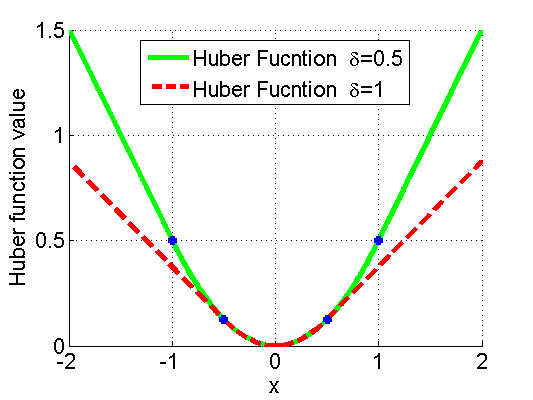
\includegraphics[width=0.2\textwidth]{figs/huber_loss}
  \end{center}
\end{wrapfigure}
\item allows construction of an estimate which allows the effect of outliers to be reduced, while treating non-outliers in a more standard way.
\item Often used in the context of robust filtering of Laplace-noise ([1],[2]).
\end{itemize}
$[1]$ Robust estimation using the Huber function with a
data-dependent tuning constant (You-Gan et al. , $2007$).\\
$[2]$ An l1-laplace robust kalman smoother (Aravkin et al. , $2011$). \\
\begin{block}{In this work} 
\begin{itemize}
\item Derive robust boosting-like algorithms directly from PAC-Bayes bounds, and analyze their properties.
\item Generalize PAC-Bayes theory to the multi-task framework. 
\item Testing the algorithms in a wide range of input noise.
\end{itemize}
\end{block}
\end{frame}


\subsection{ Laplace-like family of distributions}
\begin{frame}
\frametitle{ Laplace-like family of distributions }
\begin{itemize}
\item Let $Q(\vomega;\vmu,\vsigma)\in\LL$, then, 
\begin{align*}
Q(\vomega;\vmu,\vsigma)&= \frac{1}{2^d \prod_{k=1}^d \sigmai{k}}
e^{{-\| \vomega-\vmu \|_{\vsigma,1}} } ~,~ {\| \vomega \|}_{\vsigma,1} = \frac{1}{2d}\sum_{k=1}^{d}
\frac{ |\omega_{k}| }{\sigmai{k}}
\end{align*}

\item Uni-modal distribution with mean $\vmu$, and
 diagonal covariance matrix $\Sigma=2\times\diag{\paren{\sigma_1^2,..,\sigma_d^2}}$.
\item \textbf{Proposition:}  The single continuous $d$-dimensional distribution $Q(\vomega)$ with  a bounded expected $\vsigma$-weighted $\ell_1$-norm, $E \paren{\|
  \vomega-\vmu \|}_{\vsigma,1} \leq 1$,  which
maximizes the information-theoretic entropy maintains $Q\in LL$.
\end{itemize}
\begin{block}{Theorem 1} 
Let $\cP\paren{\vmup,\vsigmap},\cQ\paren{\vmuq,\vsigmaq}\in\LL$ 
be two LL distributions. The KL- divergence between these two distributions is well defined and given by,
\begin{align*}
\KL(\cQ \Vert \cP)  \!=&\! \sum_{k=1}^{d}\!  \Bigg[    \frac{\sigmaqi{k}}{\sigmapi{k} }\paren{ \frac{ |\muqi{k}-\mupi{k}| }{\sigmaqi{k}}+e^{{-\frac{ |\muqi{k}-\mupi{k}| }{\sigmaqi{k}} } }  }  
\!\!\!+\!\log{ \paren{ \frac{\sigmapi{k}}{\sigmaqi{k}} } }\!\!-1\! \Bigg].
%\label{kl_laplace} 
\end{align*}
%\label{DKL}
\end{block}
\end{frame}



\begin{frame}
\frametitle{ Laplace-like family of distributions }
\begin{itemize}
\item Setting $\mup=0$ and $\sigmaq=\sigmap$ in the $1$-dimensional case, We obtain,
\begin{align*}
g_{\sigma_Q}(\mu_Q)&=  \frac{|\mu_{Q}|}{\sigma_{Q}}
+\exp{\braces{-\frac{|\mu_{Q}|}{\sigma_{Q}} } }  -1 \\
   &\approx \left\{ \begin{array}{rl}
  { \frac{|\mu_{Q}|}{\sigma_{Q}}} -1~$ &\mbox{  $\abs{x}\gg 1$} \\
  \frac{1}{2}\paren{\frac{|\mu_{Q}|}{\sigma_{Q}}}^2 &\mbox{ $\abs{x}\ll1$}
       \end{array} \right.
\end{align*}
\end{itemize}
\begin{figure}
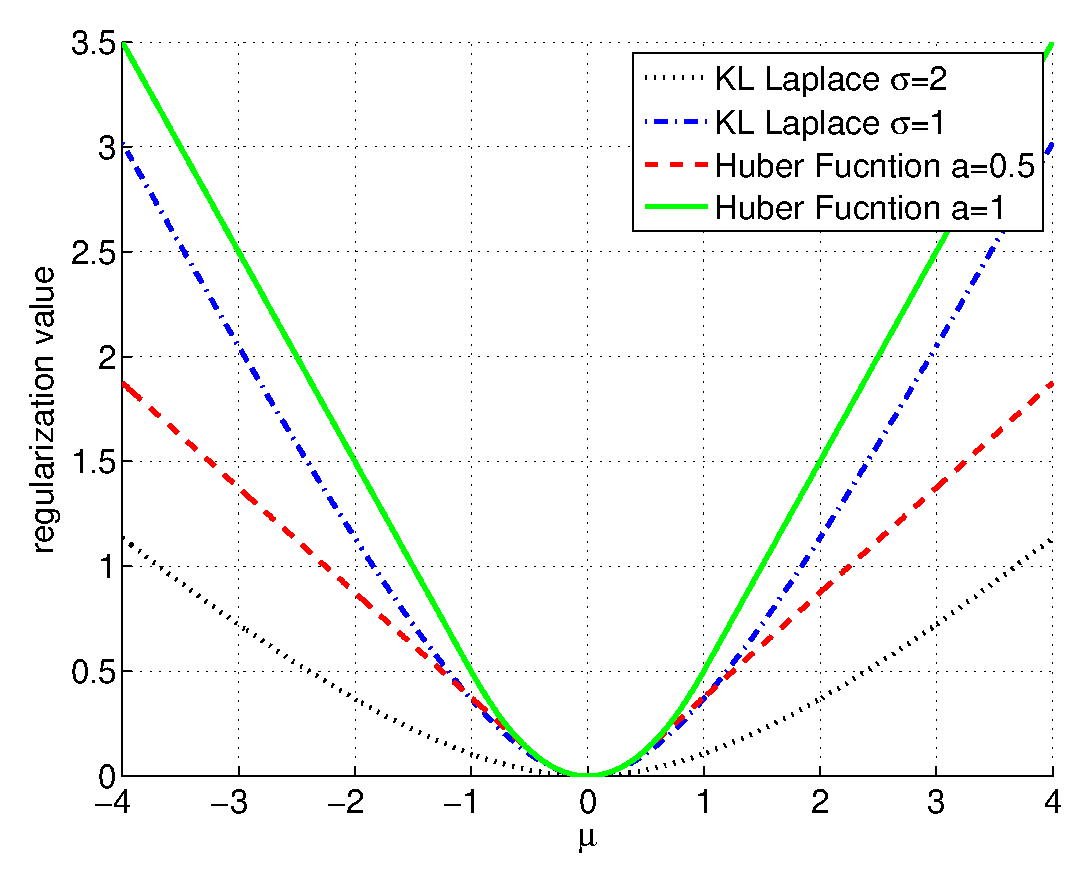
\includegraphics[width=0.2\textwidth]{figs/kl_hubber}
\end{figure}
\begin{enumerate}
\item  Huber function $\not\in C^2 ~\Longrightarrow ~g_{\sigma_Q}(\mu_Q) \in C^{\infty}$.
 \item Huber function is convex $~\Longrightarrow~ g_{\sigma_Q}(\mu_Q)$ is strictly-convex.
\item $g_{\sigma_Q}(\mu_Q)$ is closely related to the \textit{linear loss} $\elllin$  (later..) 
\end{enumerate}

\begin{block}{Theorem 1} 
Let $\cP\paren{\vmup,\vsigmap},\cQ\paren{\vmuq,\vsigmaq}\in\LL$ 
be two LL distributions. The KL- divergence between these two distributions is well defined and given by,
\begin{align*}
\KL(\cQ \Vert \cP)  \!=&\! \sum_{k=1}^{d}\!  \Bigg[    \frac{\sigmaqi{k}}{\sigmapi{k} }\paren{ \frac{ |\muqi{k}-\mupi{k}| }{\sigmaqi{k}}+e^{{-\frac{ |\muqi{k}-\mupi{k}| }{\sigmaqi{k}} } }  }  
\!\!\!+\!\log{ \paren{ \frac{\sigmapi{k}}{\sigmaqi{k}} } }\!\!-1\! \Bigg].
%\label{kl_laplace} 
\end{align*}
%\label{DKL}
\end{block}
\end{frame}




\begin{frame}
\frametitle{ Laplace-like and PAC-Bayes bounds  }
\begin{block}{Theorem 2  (PAC-Bayes for linear classifiers)} 
For any distribution $\cD$, any set $\cal H$
of classifiers, any distributions $P,Q$ of support $\cal H$, any
$\delta \in\{0,1\}$, and any positive real scalar $c$, we have:
\begin{align*}
&\Expp{\vomega\sim Q, (\vx,y)\sim \cD}{\ellzo(y(\vx\cdot\vomega))}
\leq \label{main_eq}
 \frac{1}{1-\exp(-c)}\times \\ 
 &\Bigg [ 1-   \exp\bigg\{ -\frac{1}{m}\bigg(  cE_{\vomega\sim
     Q}\brackets{\sum _{i=1}^m \ellzo(\yii(\vxii\cdot\vomega)) }
+\KL(Q \Vert P)+\ln\frac{1}{\delta}\Bigg)\bigg\}\bigg]\nonumber
\end{align*}
with probability of at least $1-\delta$.
\begin{figure}
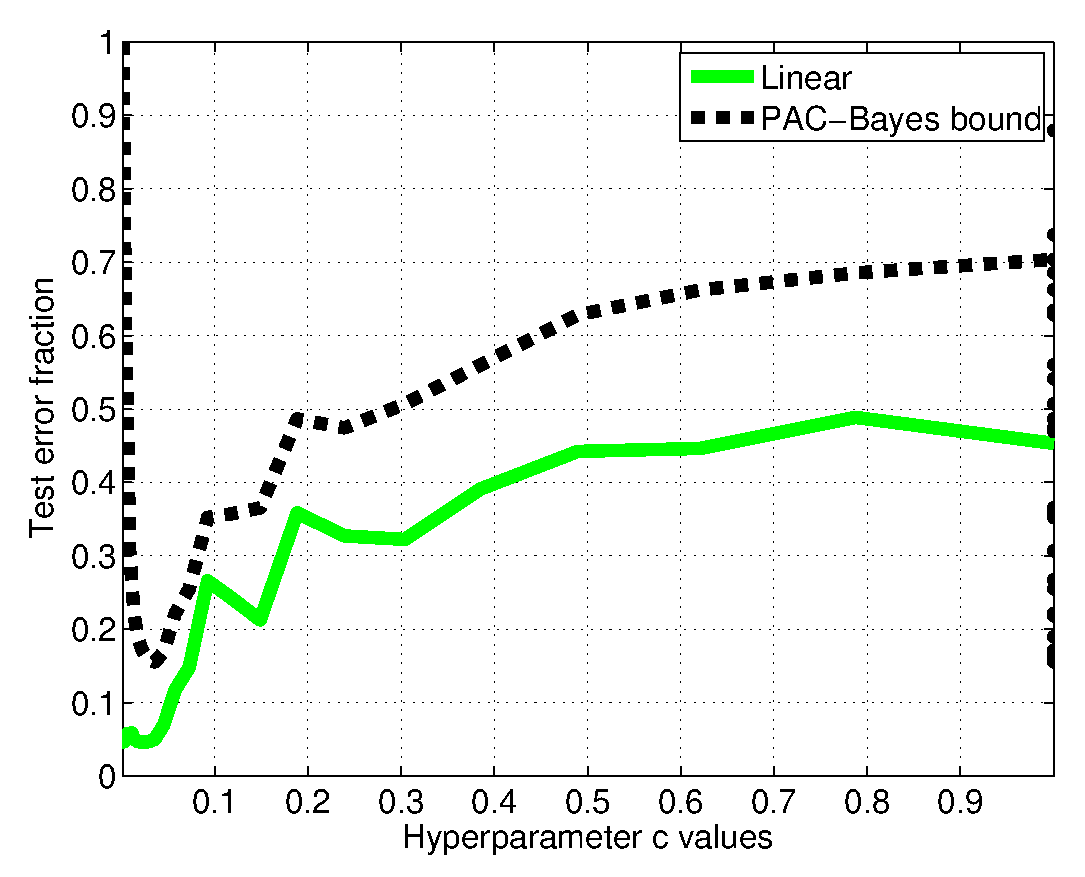
\includegraphics[width=0.2\textwidth]{figs/boundSimu}
\end{figure}
\end{block}

\begin{itemize}
\item for fixed $(c,\delta)$ and natural
initialization for  prior $(\vmup,\vsigmap)= \paren{\vzero,\vone}$,
 \begin{align*}
 \!\!\!\!\!\!\!\!\!\!\!\!\!\!\F(\vmuq,\vsigmaq)\!\!=\!\!\sum_{k=1}^{d}\!\! \paren{\!\sigmaqi{k}e^{-\frac{\abs{\muqi{k}}}{\sigmaqi{k}}}\!\!-\!\log{ \paren{
      \sigmaqi{k} } }\!\! }\!\!+\!\Vert \vmuq
\Vert_1\!+\!c\! \sum _{i=1}^m\Pr\paren{ \yii(\vxii\cdot\vomega)\leq0} 
\end{align*}
\end{itemize}
\end{frame}

\begin{frame}
\frametitle{ Laplace-like and PAC-Bayes bounds  }
\begin{itemize}
\item The error term $\Pr\paren{ \yii(\vxii\cdot\vomega)\leq0}$ is never convex for each $\vmu$.
\item Two ways to go: 
\begin{enumerate}
\item Upper-bound the error term with smooth and convex functions.
\item Directly calculate the error term,  then bound the result
with  smooth and convex functions.
\end{enumerate}
\item As we shall see later- the tighter the bound, the better the results..
\end{itemize}
\begin{figure}
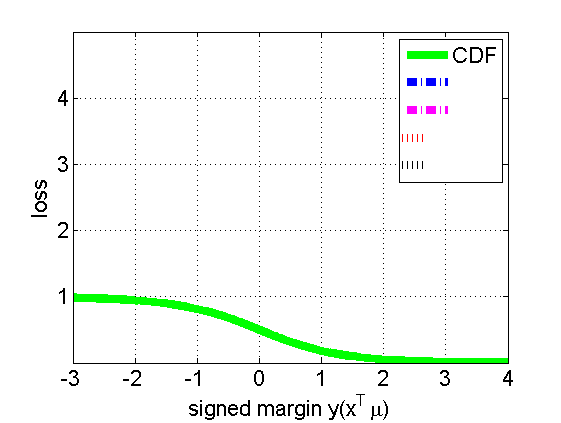
\includegraphics[width=0.4\textwidth]{figs/losses_cdf}
\end{figure}
\end{frame}


\begin{frame}
\frametitle{ The ExpLoss  }
\begin{itemize}
\item \textbf{Assumptions:}
\begin{enumerate}
\item Isotropic $\LL$ distributions, $\forall k:\sigma_{Q,k}=\sigma$.
\item Bounded input, $\max_{1\leq i\leq m}\Vert \vxii \Vert_\infty < 1$.
 \end{enumerate}
\item Consider the ExpLoss: $\ellexp\paren{y (\vomega \cdot \vx)} &= \Expp Q{e^{- y  \vx \cdot\vomega} }$.
\item Define scaled mean vector, $\mu_k=\frac{\mu_{Q,k}}{\sigma}$. The resulting objective, 
\begin{align*}
\F_{\exp} \paren{\vmu,\sigma}&=-d\log\sigma+
\sigma\sum_{k=1}^{d} \paren{\abs{\mu_{k} }+e^{-\abs{\mu_{k} } } }+ c\sum_{i =1}^m D_i e^{-\sigma \yii  \vxii \cdot \vmu},\\
&\textrm{for } D_i = D_i\paren{\vsigmaq}= \prod_{k=1}^d {\paren{1-\paren{x_{i,k}\sigmaqi{k}}^2}}^{-1}.
\label{exp_objective}
\end{align*}
\item For a fixed $\sigma$, we perform coordinate descent over $\vmu$.
\end{itemize}
\end{frame}





\begin{frame}
\frametitle{ The ExpLoss  }
\begin{itemize}
\item Define $~~C_+( \vmu^{(k)},\sigma)=c\sum_{i =1}^m D_i e^{-\sigma \yii  \vxii^{(k)} \cdot \vmu^{(k)}} \paren{  \frac{1+\sigma \yii  x_{ik}  }{2}}$  \\ $~~~~~~~~~~~C_-( \vmu^{(k)},\sigma)=c\sum_{i =1}^m D_i e^{-\sigma \yii  \vxii^{(k)} \cdot \vmu^{(k)}} \paren{  \frac{1-\sigma \yii  x_{ik}  }{2}}$
 \item For the non-regularized objective we would get,
 %\begin{align*}
 $\mu_k=0.5\ln{\paren{\frac{C_+}{C_-}}}$.
 %\end{align*}
 \end{itemize}
 
\vspace{-0.1cm}
\begin{exampleblock}{\textbf{The Huber-Reg AdaBoost algorithm} }
\begin{figure}[!h!]

{
\begin{itemize}
\item {\bf Input:} {Train set $\braces{(\vxii,\yii)}_{i=1}^m$ ,
  $\vmup\in \mathbb{R}^d$, $\vsigma\in(0,1)$, $c>0$, $T>0$.   }
\item{\bf Initialization}:$\quad\vmuq^{(1)} =\vmup \quad; \quad D_{i} ~~ \textrm {for     }~ i = 1 \comdots m$.\\
{\bf Loop} For $t = 1 \comdots T$ do:

\nolineskips
\begin{itemize}
\item 
%{ $t\leftarrow 1$ \KwTo $T$ }{
Choose coordinate: $k\in \braces{1,..,d}$,
and set: $C_+( \vmu^{(k)},\sigma)~,~ C_-( \vmu^{(k)},\sigma)$.

\item Update: 
  If {$\paren{C_+\geq C_-}$}
 \\then {$\muqi{k}^{(t+1)}\leftarrow \muqi{k}^{(t)}+  \log{\paren{ \frac{-\sigma+\sqrt{\sigma^2+4C_-(\sigma+C_+)}}{2C_-}}}  }
 \\~~~~~~~else {$\muqi{k}^{(t+1)}\leftarrow \muqi{k}^{(t)}+\log{\paren{ \frac{-\sigma+\sqrt{\sigma^2-4C_-(\sigma-C_+)}}{2(\sigma-C_+)}}}   }
%      \KwOut{$\vmu_Q^{(T+1)}$}
\end{itemize}
\item {\bf Output: $\vmu_Q^{(T+1)}$}\\}
\end{itemize}


 \end{figure}
 \end{exampleblock}
\begin{itemize}
%\item Performs better then AdaBoost, but both breaks in the presence of outliers.   
\end{itemize}
\end{frame}



\begin{frame}
\frametitle{ The LogLoss  }
\vspace{-0.1cm}
\begin{itemize}
\item Consider the LogLoss: $\elllog\paren{y (\vomega \cdot \vx)} = \log_2{\paren{
    1+\exp{\paren{-y \paren{ \vomega \cdot \vx } } } }}$,
%\item The LogLoss objective,
\begin{align*}
\!\!\!\!\!\!\!\!\!\!\!\F_{\log} &\paren{\vmuq,\vsigmaq}\!=\!\!
\sum_{k=1}^{d}\!\! \paren{\!\!\sigmaqi{k}e^{-\frac{\abs{\muqi{k}}}{\sigmaqi{k}}}\!\!-\!\log{ \paren{
      \sigmaqi{k} } } \!\!}\!\!+\!\Vert \vmuq
\Vert_1\!+\! c\!\sum_{i =1}^m \! \log_2\!\paren{1\!+\!D_i e^{- y  \vxii \cdot \vmuq}}
%\label{log_objective}
\end{align*}
\item Define the incremental change $\delta_k ^{(t)} =
\muqi{k}^{(t+1)}-\muqi{k}^{(t)}$.
\vspace{-0.15cm}
\begin{block}{Theorem 3} 
The 
difference between
the LogLoss objective %log_loss_objective} 
evaluated at time $t$ and time $t+1$ is lower bounded,
\vspace{-0.6cm}
\begin{align*}
&\F_{\log}(\vmuq^{(t)})
-\F_{\log}(\vmuq^{(t+1)}) \geq  c\sigmaqi{k} \paren{\gamma_k^{+}\brackets{1-e^{-\frac{\delta_k ^{(t)}}{\sigmaqi{k}}}}+\gamma_k^{-}\brackets{1-e^{\frac{\delta_k ^{(t)}}{\sigmaqi{k}}}}}  ~
 \\  &  +\abs{\muqi{k}^{(t)} }+\sigmaqi{k} e^{-\frac{\abs{\muqi{k}^{(t)}
      }}{\sigmaqi{k}}}-\abs{\muqi{k}^{(t)} +\delta_k^{(t)}
  }-\sigmaqi{k} e^{-\frac{\abs{\muqi{k}^{(t)} +\delta_k^{(t)}
      }}{\sigmaqi{k}}}.
\end{align*}

%\(%\begin{align*}
%\Delta_t \geq c\,\sigmaqi{k} \paren{\gamma_k^+\brackets{1-\exp\paren{-\frac{\delta_k ^{(t)}}{\sigmaqi{k}}}}+\gamma_k^-\brackets{1-\exp\paren{\frac{\delta_k ^{(t)}}{\sigmaqi{k}}}} }~,
%\)%\end{align*}
%
\vspace{-0.2cm}
  $q_t(i)\!\! =\!\! {D_i}/\!\paren{D_i\!+\!e^{\yii  \vxii \cdot \vmuq^{(t)} }},\gamma_k^{\pm} =\! \sum_{i=1}\mb{1}(\yii x_{i,k}\in\pm)q_t(i)\abs{x_{i,k}}$.
\vspace{-0.1cm}
\end{block} 
\end{itemize}
\end{frame}

\begin{frame}
\frametitle{ The LogLoss  }
\begin{itemize}
\vspace{-0.1cm}
\item omitting terms independent of $\delta_k ^{(t)}$, we can minimize the following, 
\begin{align*}
%&argmin_{\delta_k^{(t)}}\braces{ -\abs{\mu_{Q,k}^{(t)} +\delta_k^{(t)} }-e^{-\abs{\mu_{Q,k}^{(t)} +\delta_k^{(t)} }}-                     c\sigmaqi{k} \paren{\gamma_k^{+}e^{-\frac{\delta_k ^{(t)}}{\sigmaqi{k}}}+\gamma_k^{-}e^{\frac{\delta_k ^{(t)}}{\sigmaqi{k}}}}  } \\
 %=& 
\arg\min_{\delta_k^{(t)}}&\Bigg[ \abs{\mu_{Q,k}^{(t)} +\delta_k^{(t)}
  } +\sigmaqi{k} e^{-\frac{\abs{\muqi{k}^{(t)} +\delta_k^{(t)}
      }}{\sigmaqi{k}}}   +c\sigmaqi{k}\paren{\gamma_k^{+}e^{-\frac{\delta_k ^{(t)}}{\sigmaqi{k}}}+\gamma_k^{-}e^{\frac{\delta_k ^{(t)}}{\sigmaqi{k}}}}  \Bigg] ~.
%\label{argmaxLogLoss}
\end{align*}
\end{itemize}
\vspace{-0.4cm}
\begin{exampleblock}{\textbf{BaLaBoost algorithm}  [Noy and Crammer, 2014]}
\begin{figure}[!h!]

{
\begin{itemize}
\item {\bf Input:} {Train set $\braces{(\vxii,\yii)}_{i=1}^m$ ,
  $\vmup\in \mathbb{R}^d$, $\vsigma_Q\in(0,1)^d$, $c>0$, $T>0$.   }
\item{\bf Initialization}:$\quad\vmuq^{(1)} =\vmup \quad; \quad D_{i} ~~ \textrm {for     }~ i = 1 \comdots m$.\\
{\bf Loop} For $t = 1 \comdots T$ do:

\nolineskips
\begin{itemize}
\item 
%{ $t\leftarrow 1$ \KwTo $T$ }{
Choose coordinate: $k\in \braces{1,..,d}$,
and set: $\gamma_k^{+}~,~ \gamma_k^{-}$.

\item Update: 
  If {$\paren{\gamma_k^{+}\exp{\braces{{\frac{2\muqi{k}^{(t)}  }{\sigmaqi{k}}}}}\geq\gamma_k^{-}}$}
 \\then {$\muqi{k}^{(t+1)}\leftarrow \muqi{k}^{(t)}+\delta^{(t)}_{k,+}(\gamma_k^{+},\gamma_k^{-},\muqi{k},\sigmaqi{k})  }
 \\~~~~~~~else {$\muqi{k}^{(t+1)}\leftarrow \muqi{k}^{(t)}+\delta^{(t)}_{k,-}(\gamma_k^{+},\gamma_k^{-},\muqi{k},\sigmaqi{k})   }
%      \KwOut{$\vmu_Q^{(T+1)}$}
\end{itemize}
\item {\bf Output: $\vmu_Q^{(T+1)}$}\\}
\end{itemize}


 \end{figure}
 \end{exampleblock}
\end{frame}




\begin{frame}
\frametitle{ The LogLoss  }
\begin{itemize}
\item omitting terms independent of $\delta_k ^{(t)}$, we can minimize the following, 
\begin{align*}
%&argmin_{\delta_k^{(t)}}\braces{ -\abs{\mu_{Q,k}^{(t)} +\delta_k^{(t)} }-e^{-\abs{\mu_{Q,k}^{(t)} +\delta_k^{(t)} }}-                     c\sigmaqi{k} \paren{\gamma_k^{+}e^{-\frac{\delta_k ^{(t)}}{\sigmaqi{k}}}+\gamma_k^{-}e^{\frac{\delta_k ^{(t)}}{\sigmaqi{k}}}}  } \\
 %=& 
\arg\min_{\delta_k^{(t)}}&\Bigg[ \abs{\mu_{Q,k}^{(t)} +\delta_k^{(t)}
  } +\sigmaqi{k} e^{-\frac{\abs{\muqi{k}^{(t)} +\delta_k^{(t)}
      }}{\sigmaqi{k}}}   +c\sigmaqi{k}\paren{\gamma_k^{+}e^{-\frac{\delta_k ^{(t)}}{\sigmaqi{k}}}+\gamma_k^{-}e^{\frac{\delta_k ^{(t)}}{\sigmaqi{k}}}}  \Bigg] ~.
%\label{argmaxLogLoss}
\end{align*}
\end{itemize}
\begin{exampleblock}{\textbf{BaLaBoost algorithm}  [Noy and Crammer, 2014]}
\begin{figure}[!h!]

{
\begin{itemize}
\item {\bf Input:} {Training set $\braces{(\vxii,\yii)}_{i=1}^m$ ,
  $\vmup\in \mathbb{R}^d$, $\vsigma_Q\in(0,1)^d$, $c>0$, No. of iterations $T$.   }\\
\item{\bf Initialization}:$\quad\vmuq^{(1)} =\vmup \quad; \quad D_{i} ~~ \textrm {for   } i = 1 \comdots m
$\\
{\bf Loop} For $t = 1 \comdots T$ do:

\nolineskips
\begin{itemize}
\item 
%{ $t\leftarrow 1$ \KwTo $T$ }{
Choose coordinate: $k\in \braces{1,..,d}$,
and set: $\gamma_k^{+}~,~ \gamma_k^{-}$.

\item Update: 
  If {$\paren{\gamma_k^{+}\exp{\braces{{\frac{2\muqi{k}^{(t)}  }{\sigmaqi{k}}}}}\geq\gamma_k^{-}}$}
 \\then {$\muqi{k}^{(t+1)}\leftarrow \muqi{k}^{(t)}+  \sigmaqi{k} \log{\paren{ \frac{1+\sqrt{1+4c\gamma_k^{-}\brackets{\exp{\braces{-\frac{\muqi{k}^{(t)} }{\sigmaqi{k}}} }+c\gamma_k^{+}} }}{2c\gamma_k^{-}}                    }}$}
 \\else {$\muqi{k}^{(t+1)}\leftarrow \muqi{k}^{(t)}+  \sigmaqi{k} \log{\paren{ \frac{1+\sqrt{1+4c\gamma_k^{+}\brackets{\exp{\braces{\frac{\muqi{k}^{(t)} }{\sigmaqi{k}}} }+c\gamma _k^{-}} }}{2 \brackets{\exp{\braces{\frac{\muqi{k}^{(t)} }{\sigmaqi{k}}} }+c\gamma_k^{-}}    }                    }}$
      }
%      \KwOut{$\vmu_Q^{(T+1)}$}
\end{itemize}
\item {\bf Output: $\vmu_Q^{(T+1)}$}\\}
\end{itemize}


 \end{figure}
 \end{exampleblock}
\end{frame}

\end{document}
